
Diese Hypothese geht davon aus, dass sich der Schnee bei mechanische Anregung von einem festen in den flüssigen Zustand übergeht. Ob der Übergang stattfindet oder nicht, könnte vom LWC Wert abhängen.

Um die Idee zu testen, wird ein vibrierendes Objekt mit hoher Dichte auf den Schnee gelegt, und es wird beobachtet, wie sich das Objekt durch den Schnee bewegt.

Die Form und der Name des Objekts wurde vom AvaNode inspiriert. Der AvaNode ist eine laufende Produktentwicklung des Instituts IPEK der OST mit dem Lawinenhänge überwacht werden sollen. Der für das Objekt und Verfahren gewählte Name ist VibraNode. Für die Umsetzung wurde ein Morphologischer Kasten mit drei Varinanten erstellt.


\begin{figure}[H]
    \centering
    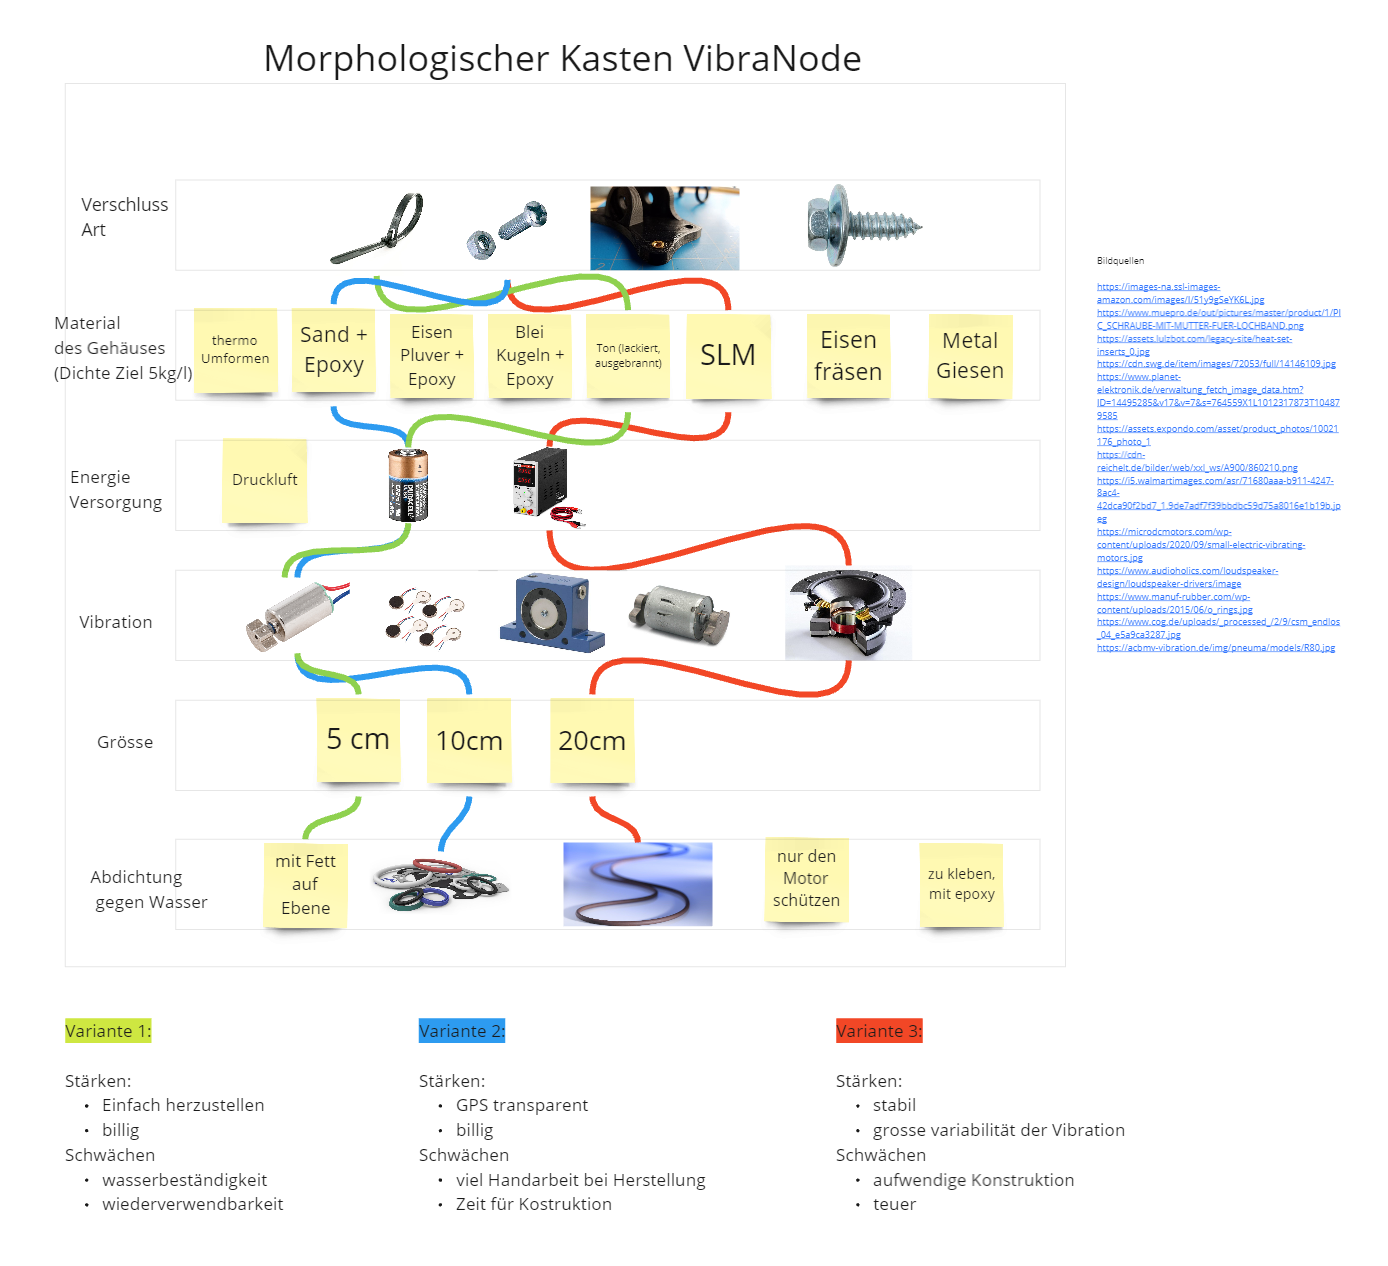
\includegraphics[width=0.9\textwidth]{Bilder/Unbenann2t.PNG}
    \caption{Morphologischer Kasten für VibraNode}
    \label{fig:Bildverarbeitnugskonzpet}
\end{figure}




Die in Abbildung \ref{fig:Bildverarbeitnugskonzpet} dargestellte Variante 1 wurde gewählt, da die Umsetzung und somit das Testen einfach ist. Die Schwächen, wie die fehlende Wiederverwendbarkeit, sind hier in der Vorstudie noch nicht gravierend. Die Schwäche der Wasserbeständigkeit wurde mit einer passenden Beschichtung gelöst.

Für den Test mit dem VibraNode wird der VibraNode auf die Schneedecke gelegt. Das Messergebniss ist, ob sich der VibraNode im Schnee versinckt.

Die Testergebnisse fielen negativ aus. Der VibraNode konnte trotz seiner Dichte von 1600 kg/m3 nicht in den Schnee eindringen. Auch wenn der Schnee wurde mit flüssigem Wasser gesättigt war. Damit  stellt sich die neue Frage, ob der LWC einen kausalen oder nur einen korrelativen Zusammenhang mit Gleitschneelawinen hat, und wie weit die Vorgeschichte und andere Faktoren des Schnees mitbetrachtet werden muss. \cite{Altman.2015}
